\documentclass[a4paper]{article}
\usepackage{yibin}

%-----------------------------------------BEGIN DOC----------------------------------------

\begin{document}
\renewcommand{\contentsname}{目\ 录}
\renewcommand{\appendixname}{附录}
\newcommand{\appendixpagename}{附录}
\renewcommand{\refname}{参考文献} 
\renewcommand{\figurename}{图}
\renewcommand{\tablename}{表}
\renewcommand{\today}{\number\year 年 \number\month 月 \number\day 日}

\begin{figure}
    \centering
    
\includegraphics[width=0.5\linewidth]{images/logo.png}
\end{figure}


% 封面
\title{{\Huge 信息类实验报告模板{\large\linebreak\\}}{\Large 实验题目:\linebreak\linebreak}}
\author{\\
姓\ 名: xxxxxx\\
学\ 号: xxxxxx\\
班\ 号: 人工智能2201\\
课\ 程: xxxxxx\\
授\ 课\ 教\ 师: xxxxxx\\\\
东北大学\\
信息科学与工程学院\\
}
\date{\today}
\maketitle
\newpage

%-----------------------------------------ABSTRACT-------------------------------------
\begin{center}
{\Large\bf{摘\ 要\\}}
\end{center}
请在此处输入摘要内容,摘要应简要说明实验目的、实验方法、主要结果以及结论。摘要通常为150-200字。


\textcolor{red}{!!!注意摘要如果不需要的话把这段注释掉即可}

\textbf{关键词}:抑郁风险预测,堆叠集成学习,XGBoost,CatBoost,LightGBM,Logistic Regression,特征工程,超参数优化,消融实验

\newpage


%-----------------------------------------CONTENT-------------------------------------
\begin{center}
\tableofcontents\label{c}
\end{center}
\newpage

%------------------------------------------TEXT--------------------------------------------
\section{实验概述}

在这一部分中,简要介绍实验背景、目的、涉及的基本原理与实验内容。可以包括:
\begin{itemize}
    \item 实验目的
    \item 实验背景
    \item 实验基本原理
\end{itemize}

\section{实验原理与方法}

这一部分详细描述实验过程中涉及的理论原理和方法,包括可能用到的公式推导、实验步骤的描述,图示或流程图等。

这是一个控制工程中传递函数的单行公式示例:$G(s) = \frac{Y(s)}{U(s)}$。

这是一个PID控制器的独立公式示例:
\[
G_{\text{PID}}(s) = K_p + K_i \frac{1}{s} + K_d s
\]


这是控制系统闭环传递函数的公式:
\[
T(s) = \frac{G(s)}{1 + G(s)H(s)}
\]
s
其中,$G(s)$ 是开环传递函数,$H(s)$ 是反馈函数。


\subsection{实验平台及环境}
描述实验所用的软件、硬件平台等。包括:
\begin{itemize}
    \item 编程语言/工具(如MATLAB, Python等)
    \item 计算设备(如CPU、GPU等硬件配置)
    \item 实验环境(如操作系统,开发环境)
\end{itemize}

\section{实验步骤}

在这一节详细描述实验具体步骤,分阶段说明实验实施的过程:
\begin{itemize}
    \item 数据输入与预处理
    \item 实验中各个模块的功能描述
    \item 算法设计与实现
\end{itemize}

代码块按以下格式插入:

进入项目的根目录(假设为 \texttt{\~{}/a\_star}),并使用 \texttt{catkin\_make} 命令编译项目。具体步骤如下:

\begin{myblock}{编译项目}
\begin{verbatim}
cd ~/a_star
catkin_make
\end{verbatim}
\end{myblock}

\begin{myblock}{程序报错}
\begin{verbatim}
a_star: /home/leon/a_star/src/a_star/include/a_star/spline.h:288: 
void {anonymous}::tk::spline::set_points(const std::vector<double>&, 
const std::vector<double>&, bool): 
Assertion `x.size()>2' failed.
已放弃 (核心已转储)
\end{verbatim}
\end{myblock}

\section{实验结果与分析}

展示实验的结果,包括表格、数据或图示。需要对实验结果进行详细分析和解释,解释为何得出此结论,如图\ref{fig:equipment_diagram},表格\ref{tab:comparison}。

在LaTex写作时,输入引号时并非直接用键盘上的引号键
引号的正确输入:
左引号:按一次 ` (即主键盘区左上角,Tab键上方的键)。
右引号:按一次 ' (即分号右,回车左的键)。
wrong 'example'
correct `example'

\subsection{图片示例}

\begin{figure}[H]
    \centering
    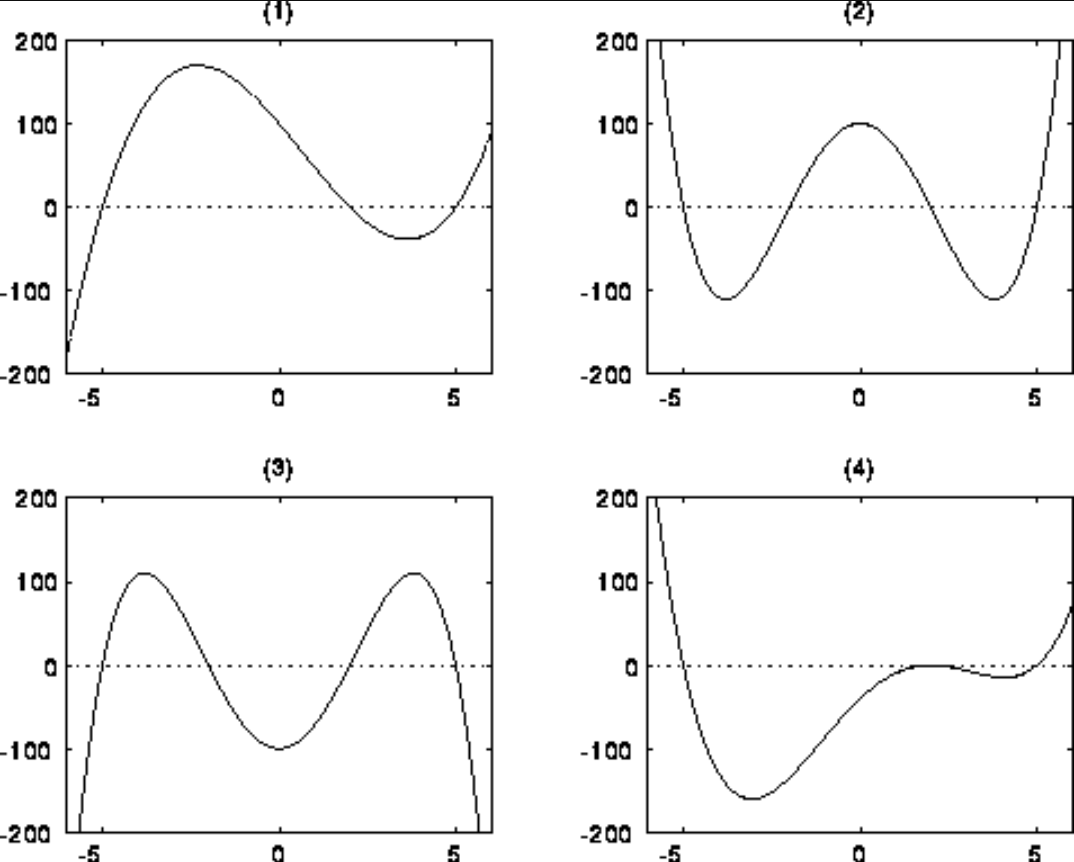
\includegraphics[width=0.7\linewidth]{images/plot.png}
    \caption{实验设备示意图}
    \label{fig:equipment_diagram}
\end{figure}

\subsection{子图示例}

\begin{figure}[H]
    \centering
    \begin{subfigure}[b]{0.4\textwidth}
        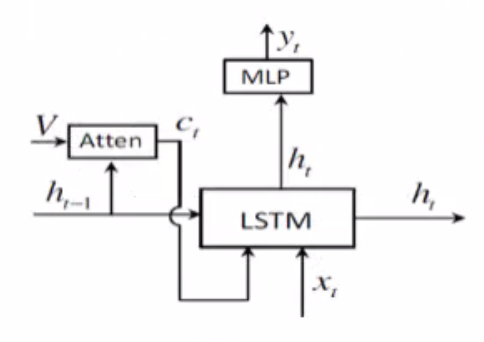
\includegraphics[width=\textwidth]{images/image1.png}
        \caption{子图1}
        \label{fig:sub_image1}
    \end{subfigure}
    \hfill
    \begin{subfigure}[b]{0.4\textwidth}
        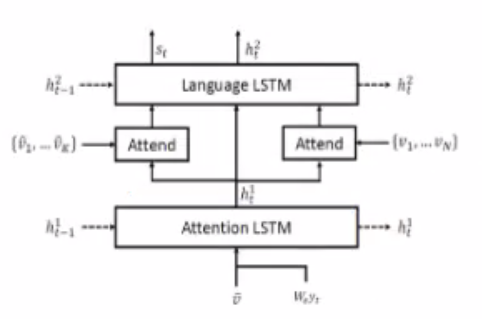
\includegraphics[width=\textwidth]{images/image2.png}
        \caption{子图2}
        \label{fig:sub_image2}
    \end{subfigure}
    \caption{实验结果对比图}
    \label{fig:comparison}
\end{figure}

\subsection{表格示例}

\begin{table}[H]
    \centering
    \begin{tabular}{l|c|c}
    \toprule
    项目 & 实验组1 & 实验组2 \\
    \midrule
    测量值1 & 23.5 & 24.1 \\
    测量值2 & 30.2 & 29.8 \\
    测量值3 & 22.1 & 21.9 \\
    \bottomrule
    \end{tabular}
    \caption{实验数据对比表}
    \label{tab:comparison}
\end{table}

\subsection{参考文献引用示例}
在进行实验时,我们使用了相关研究的理论模型,例如 \cite{example1}。

% --------------------------------Evaluation----------------------------------------
\section{结论}

总结实验的主要发现,讨论实验的结果是否达到预期目标,指出实验中的不足和进一步改进的方向。

% -----------------------------------Appendix----------------------------------------
\appendix
\section{代码}\label{sub:app.code}

展示实验中用到的主要代码,附上详细注释以方便理解。

\subsection{MATLAB 代码示例}

\begin{lstlisting}[language=Matlab, caption={MATLAB 代码示例}, label={code:matlab_example}]
% 这是一个简单的MATLAB代码示例
x = 0:0.01:2*pi; % 定义x为0到2*pi之间的100个点
y = sin(x); % 计算sin(x)的值

% 绘制图像
figure;
plot(x, y);
title('正弦函数曲线');
xlabel('x');
ylabel('sin(x)');
grid on;
\end{lstlisting}

\subsection{Python 代码示例}

\begin{lstlisting}[language=Python, caption={Python 代码示例}, label={code:python_example}]
# 这是一个简单的Python代码示例
import numpy as np
import matplotlib.pyplot as plt

x = np.linspace(0, 2*np.pi, 100) # 生成0到2*pi的100个点
y = np.sin(x) # 计算sin(x)

# 绘制图像
plt.plot(x, y)
plt.title('正弦函数曲线')
plt.xlabel('x')
plt.ylabel('sin(x)')
plt.grid(True)
plt.show()
\end{lstlisting}

\subsection{C++ 代码示例}

\begin{lstlisting}[language=C++, caption={C++ 代码示例}, label={code:cpp_example}]
#include <iostream>
using namespace std;

int main() {
    // 输出Hello World
    cout << "Hello, World!" << endl;

    // 简单的循环
    for (int i = 0; i < 5; i++) {
        cout << "这是第 " << i+1 << " 次循环" << endl;
    }

    return 0;
}
\end{lstlisting}



\newpage
% -----------------------------------REFERENCE----------------------------------------
\begin{thebibliography}{9}
\bibitem{example1} 某某作者, \emph{书名或文章名}, 出版社或期刊, 年份, 页码.
\bibitem{example2} John Doe, \emph{Title of the paper or book}, Journal or Publisher, Year, Pages.
\bibitem{quigley2009} Quigley, M., et al., \emph{ROS: an Open-Source Robot Operating System}, ICRA Workshop on Open Source Software, 2009.
\bibitem{thrun2005} Thrun, S., Burgard, W., \& Fox, D., \emph{Probabilistic Robotics}, MIT Press, 2005.
\end{thebibliography}
\end{document}
